\section{Diskussion der Ergebnisse}
\subsection{Bewertung des Prototyps}
Zur methodischen Erstellung eines Prototyps gehört auch, diesen strukturiert zu bewerten. Ziel der Methode war es, Erkenntnis über den technischen Prozess der Implementierung einer \ac{EDA} zu erlangen und zu zeigen, dass dies im gegebenen Softwareumfeld überhaupt möglich ist. 
Gezeigt wurde zuerst einmal, dass es möglich ist, eine \ac{EDA} zu implementieren. Die Erkenntnis bezüglich des technischen Prozesses ist unter Abschnitt \ref{implementierung} dokumentiert. Hierzu muss aber erwähnt werden, dass die beschriebenen Schritte nur für ein relativ spezifisches System Gültigkeit haben. Voraussetzung ist, dass ein SAP On-Premise System sowohl als Producer als auch als Subscriber dienen soll und als Event-Platform der \ac{BTP}-Service Event Mesh verwendet werden soll. Das Beispiel deckt beispielsweise weder die Möglichkeit ab, externe Producer zu registrieren, noch ein SAP S/4 Cloud System als Subscriber zu verwenden. 
Trotzdem kann die gewonnene Erkenntnis auch in anderen Szenarien teilweise wiederverwendet werden, da die verwendeten Softwarekomponenten im Sinne der \ac{EDA} prinzipbedingt modular verwendet werden können und somit auch die Implementierung in anderen Szenarien in der beschriebenen Form wiederkehrt.
Der praktische Nutzen des Prototyps besteht also in seiner Funktion als Demo von \ac{EDA} für das vorliegende System, könnte aber auch darüber hinaus noch Anwendung finden. Aus methodischer Perspektive hat der Prototyp seinen Zweck insofern erfüllt, als das er Aufschluss über Implementierungsschritte gegeben hat, im Folgenden kann er aber auch als Grundlage für eine weitere Diskussion der Forschungsfrage dienen.

\subsection{Beurteilung von EDA und REST im Kontext des Anwendungsbeispiels}
Die Fragestellung der Arbeit war, ob es sich lohnt, die \ac{EDA} in komplexen Softwareumfeldern einzusetzen. In den theoretischen Grundlagen der Arbeit wurden einige Vorteile dieses Architekturansatzes dargestellt, die im Prototypen überprüft werden können. Konkret sollen folgende Vorteile überprüft werden:
\begin{itemize}
    \item Modularisierung
    \item Ausfallsicherheit
    \item Integrationsmöglichkeiten
\end{itemize}
\subsubsection*{Modularisierung}
Die Modularisierung ist ein zentraler Vorteil der \ac{EDA}. Durch die lose Kopplung der Komponenten und die Verwendung von Events als einheitliche Schnittstelle wird die Komplexität der Software veringert. Dieser Vorteil tritt im Prototypen in der Entkopplung der Producer und Subscriber Applikationen zutage. Hierbei wurden das \ac{BO}, welches das Ereignis produziert vollständig unabhängig von der Subscriber Applikation entwickelt. Es gibt keine Überschnitte bezüglich der Code-Basis, aber auch zeitlich wurden die beiden Komponenten unabhängig voneinander entwickelt. Es ist also durchaus auch denkbar, dass, wenn verschiedenen Teams an der Entwicklung der Anwendungen beteiligt sind, diese ohne größere Abstimmung, also unabhängig entwickeln könnten. Das ist ein großer Vorteil, da es die Entwicklungsgeschwindigkeit erhöht und die Komplexität der Software reduziert.
\subsubsection*{Ausfallsicherheit}
Aus der Modularisierung folgt logisch auch eine höhere Ausfallsicherheit der Software. In der Entwicklung trat das hervor, als beide Softwarekomponenten vollständig unabhängig voneinander getestet werden konnten, ohne dass sie aufeinander Einfluss nehmen mussten. Durch die Möglichkeit, in der Event-Platform Ereignisse zu Testzwecken auszulösen, konnten das Verhalten der Applikationen getestet werden, ohne dass eine Abhängigkeit zu anderen Komponenten bestand. Dieses Beispiel zeigt, dass, selbst wenn eine Softwarekomponente nicht läuft, die andere davon nicht beeinträchtigt wird. Im Beispiel könnte also der vom \ac{BO} bereitgestellte Service weiterlaufen, auch wenn die vom Subscriber bereitgestellte Funktionen ausfallen. Es könnten also weiterhin Travel-Objekte angelegt, geändert und gespeichert werden, es würden nur keine Benachrichtigungen mehr gesendet und die Ereignisse nicht mehr persistiert werden. Das erhöht die Verfügbarkeit des Dienstes, weil nicht jeder einzelne Fehler unbedingt zum Totalausfall des Systems führt.
\subsubsection*{Integrationsmöglichkeiten}
Die Integrationsmöglichkeiten sind ein weiterer Vorteil der \ac{EDA}. In der Implementierung des Prototyps ist die Sprache auf den Cloud-Events Standard gekommen, der in der Industrie übergreifend verwendet wird. Nativ bietet das SAP-Event Mesh die Möglichkeit, über eine API oder sogenannte Webhooks auch externe Komponenten anzubinden. In der Entwicklung des Prototyps wurde diese Möglichkeit nicht weiter getestet, die Recherche hat aber immer wieder gezeigt, dass die Integrationsmöglichkeiten des Event-Mesh sehr umfangreich sind. Als externe Quellen für Ereignisse kommen alle Anbieter infrage, die dem Standard der Cloud Events folgen. Denkbar sind beispielsweise eine Integration mit maßgeschneiderten Cloud-Anwendungen, die auf der Google Cloud Plattform oder AWS laufen.

\subsection{Chancen der Technologie im betriebswirtschaftlichen Kontext}
Als abschließende Überlegung zu dem Thema sollen die bisherigen Erkenntnisse auf einen umfassenderen Rahmen übertragen werden und aus betriebswirtschaftlicher Sicht bewertet werden.
\subsubsection*{Softwarekomplexität}
In der Entwicklung von Software in komplexen Softwareumfeldern mit vielen Komponenten und Abhängigkeiten ist \ac{EDA} ein Architekturansatz, der erheblich zur Wirtschaftlichkeit eines Projekts beitragen kann. Häufig entstehen Kosten in Softwareprojekten durch die Komplexität der Softwarearchitektur. Mit komplexen Abhängigkeiten geht erhebliche Koordinierungsarbeit in den Entwicklungsteams einher und auch das nachträgliche Ändern von Schnittstellen oder nur das Hinzufügen von zusätzlicher Funktionalität zieht häufig einen hohen Aufwand nach sich. Schlussendlich wird durch diese Komplexität die Weiterentwicklung der Software und somit des Produktes behindert.
In der Konzeptionsphase, also im Rahmen von Architekturüberlegungen können solche Probleme antizipiert und reduziert werden. Mit \ac{EDA} wurde ein Ansatz der Softwarearchitektur vorgestellt, der, wenn er stringent implementiert ist, dazu führt, dass Komponenten lose gekoppelt sind und somit die beschriebenen Abhängigkeiten reduziert werden können. Die Modularisierung der Softwarearchitektur, die durch \ac{EDA} gefördert wird, führt also dazu, dass die Komplexität der Software reduziert wird.
\subsubsection*{Agilität}
Der zweite große Vorteil der \ac{EDA} im geschäftlichen Kontext liegt darin, dass er Systeme agiler macht und diese befähigt schneller zu reagieren. Die asynchrone Verarbeitung von Ereignissen führt dazu, dass schneller auf Geschäftsvorfälle reagiert werden kann. Das liegt daran, dass in der Verarbeitung von diesen Ereignissen nicht mehr jede Systemkomponente auf einmal beansprucht wird, sondern immer nur die Komponente die wirklich zur Verarbeitung gebraucht wird, also die Subscriber. So werden parallelisierte Prozesse möglich, was die allgemeine Verarbeitungsgeschwindigkeit schon auf architektonischer Ebene erhöht. Die Event-Platform, die im Verarbeitungsprozess jedes Ereignisses eine Rolle spielt, ist hierbei meist ein hoch spezialisiertes System, dass sich mit nicht mehr als der korrekten Weiterleitung der Ereignisse befassen muss. Für diese Aufgabe wird keine inhaltliche Verarbeitung der Ereignisse benötigt, es reicht der Blick auf die mitgelieferten Meta-Daten. Somit ist auch dieses System meist sehr performant. \\
Alles in allem kommt die Einführung einer \ac{EDA} meist mit dem Versprechen daher, Ereignisse in Echtzeit verarbeiten zu können. In der Praxis hängt die Verarbeitungsgeschwindigkeit natürlich an einer Reihe von Faktoren, aus betriebswirtschaftlicher Sicht liegt in diesem Versprechen trotzdem ein großer Wert. Eine schnelle Verarbeitung von Geschäftsvorfällen bringt einen greifbaren Wettbewerbsvorteil, da Prozesse schneller ablaufen und auch auf Unvorhergesehenes zeitnaher reagiert werden kann.
\subsubsection*{Adoptionsrate in der Industrie}
In einer 2021 von solace beauftragen Studie zur Nutzung von \ac{EDA} in der Industrie wurde festgestellt, dass 85\% der befragten Unternehmen bereits \ac{EDA} einsetzen oder planen dies in Zukunft zu tun. Prioritäten, die die Einführung von \ac{EDA} vorantreiben sind demnach die Verbesserung der Kundenerfahrung, die Verbesserung der Responsivität der Systeme und die Verbesserung der Softwareresilienz. \cite[Vgl.][]{solace2021} Eine für die betriebswirtschaftliche Perspektive besonders interessante Metrik, die die Studie erhoben hat ist außerdem die Abwägung zwischen Kosten und Nutzen, wie in Abbildung \ref{solace} dargestellt. Demnach ist auch aus pragmatischer Kosten-Nutzen Perspektive die Einführung von \ac{EDA} interessant. Zur Quelle bleibt anzumerken, dass es sich bei solace um ein Unternehmen handelt, welches selbst die Verwendung von \ac{EDA} vorantreibt und somit ein Interesse an der Verbreitung dieser Technologie hat.  Methodisch bildet eine repräsentative Umfrage mit 840 Teilnehmern die Grundlage der Studie.
\begin{figure}
    \centering
    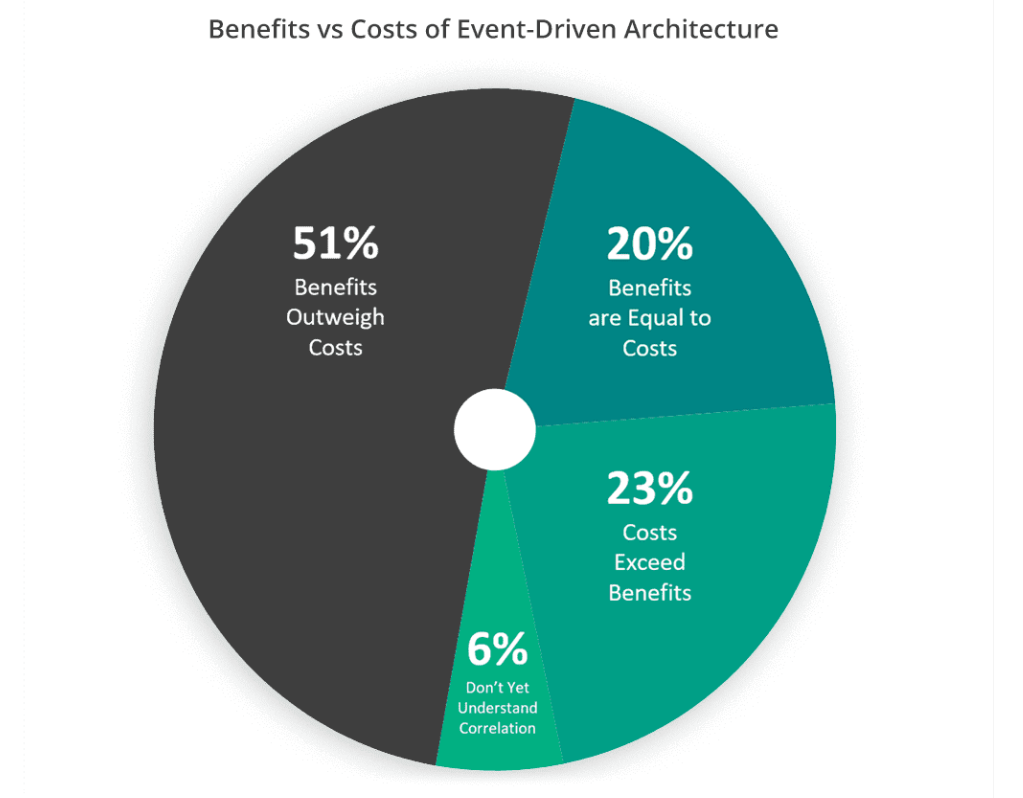
\includegraphics[width=0.85\textwidth]{solace study.png}
    \caption[Kosten und Nutzen von EDA nach einer Studie von solace]{Kosten und Nutzen von EDA nach einer Studie von solace \cite[Vgl.][]{solace2021}}
    \label{solace}
  \end{figure}
Als schließendes Argument könnte geführt werden, dass eine relativ hohe Adoptionsrate in der Industrie dazu führt, dass die Technologie weiter ausreift, mehr Praxisbeispiele und fertige Software zur Verfügung steht. Gängige Cloud-Anbieter wie AWS \cite[Vgl.][]{aws2023}, Azure \cite[Vgl.][]{azure2023}, Google Cloud \cite[Vgl.][]{gcp2021} und eben SAP bieten alle Dienste an, die als Event-Platform fungieren können und somit nativ ins Cloud-Ökosystem integriert werden können. \ac*{EDA} ist also bei weitem keine architektonisch verspielte Nischenlösung mehr, sondern bei Architekturüberlegungen ein ernst zu nehmender Ansatz, der einige Vorteile mit sich bringen kann.